\documentclass[11pt,twoside]{rmta2010esp}% For English, use rmta2010eng.cls instead of rmta2010esp.cls
%\pagestyle{myheadings} 
\usepackage[english, spanish]{babel}
\usepackage{fancyhdr}
\usepackage[utf8]{inputenc} % En caso de usar tildes, y otros caracteres especiales



\pagestyle{fancy}
\fancyhead{}
\fancyhead[RE]{\thepage \hfill {\sc r. r\'{i}os -- a. rib\'{o} -- r. mej\'{i}a -- g. molina }}
\fancyhead[LO]{{\sc Combining neural networks and geostatistics for landslide hazard assessment of San Salvador Metropolitan Area, El Salvador } \hfill \thepage}
\fancyfoot{}
\fancyfoot[RE]{{\scriptsize{\it Rev.Mate.Teor.Aplic.} (ISSN 1409-2433) {Vol. 19}(1): 1--10, January 2012}}
\fancyfoot[LO]{{\scriptsize{\it Rev.Mate.Teor.Aplic.} (ISSN 1409-2433) {Vol. 19}(1): 1--10, January 2012}}
\paginas{1}{10} % Numeros de pgina, la versión final la pone el editor; Page numbers, the Editor puts the final numbers
\usepackage{amsmath}
\usepackage{amssymb}
\usepackage{graphics}
\usepackage{graphicx} % En caso de usar figuras, con formato .esp; In case of using figures, with format .eps
\usepackage{float} 
\usepackage{url}
\usepackage{amsfonts}
\usepackage{amsmath}
\usepackage{enumerate}
\usepackage{authblk}
\usepackage{hyperref}
\usepackage{textcomp}

\DeclareGraphicsExtensions{.bmp,.png,.pdf,.jpg,.eps}



\renewcommand{\refname}{References} 



\begin{document}

\selectlanguage{spanish}
\title{Combining neural networks and geostatistics for landslide hazard assessment of San Salvador Metropolitan Area, El Salvador 
\newline
\newline
Combinando redes neuronales y geoestad\'{i}stica para evaluaci\'{o}n de deslizamientos de tierra del \'{a}rea Metropolitana de San Salvador, El Salvador}

\author[1]{Ricardo R\'{i}os \thanks{ricardo.sv@gmail.com}}
\author[2]{Alexandre Rib\'{o} \thanks{alexandre4rt@gmail.com}}
\author[3]{Roberto Mej\'{i}a \thanks{robertomejia1685@gmail.com}}
\author[4]{Giovanni Molina \thanks{giova.molina@gmail.com}}

\affil[1]{Department of Mathematics, Science and Mathematics Faculty, University of El Salvador, El Salvador.}
\affil[2]{National Institute of Health, Ministry of Health of El Salvador, El Salvador.}
\affil[3]{National Institute of Health, Ministry of Health of El Salvador, El Salvador.}
\affil[4]{Ministry of Environment and Natural Resources of El Salvador.}



\maketitle



\selectlanguage{spanish}
\begin{resumen}
Esta contribuci\'{o}n describe la creaci\'{o}n de un modelo de evaluaci\'{o}n de deslizamiento de tierra para el \'{A}rea Metropolitana de San Salvador, departamento de El Salvador. El an\'{a}lisis inicio con la obtenci\'{o}n de una foto \'{a}rea del MARN (Ministerio de Medio Ambiente y Recursos Naturales) con un total de 939407 puntos georeferenciados con el fin de producir un inventario de deslizamiento. En esta evaluaci\'{o}n de los deslizamientos se uso 4792 eventos previamente foto-interpretados y 7 factores condicionantes incluyendo: geomorfolog\'{i}a, geolog\'{i}a, precipitaciones m\'{a}ximas, aceleraciones s\'{i}smicas, pendiente del terreno, distancia a carretera y falla geol\'{o}gica. Redes Neuronales Artificiales (RNA) fueron usadas para la evaluaci\'{o}n de la susceptibilidad a deslizamiento de tierra, logrando que m\'{a}s del 80\% de deslizamientos fueran apropiadamente clasificados usando un criterio dentro y fuera de la muestra con la que se estimaron los par\'{a}metros del modelo. Regresi\'{o}n Log\'{i}stica fue usada como base de comparaci\'{o}n, obteniendo este modelo un rendimiento inferior que el de RNA con un porcentaje de correcta clasificaci\'{o}n abajo del 70\%. Para completar el an\'{a}lisis se realizo la interpolaci\'{o}n de puntos usando el m\'{e}todo kriging proveniente del enfoque geoestad\'{i}stico. Finalmente, los resultados muestran que es posible obtener un mapa de riesgo a deslizamiento de tierra, haciendo uso de una combinaci\'{o}n de RNA y t\'{e}cnicas geoestad\'{i}sticas con lo cual la presente investigaci\'{o}n puede ayudar a la mitigaci\'{o}n de deslizamientos de tierra en El Salvador.
\end{resumen}

\PC deslizamiento de tierra, evaluaci\'{o}n de riesgo, El Salvador, RNA, geoestad\'{i}stica.

\begin{abstract}
This contribution describes the creation of a landslide hazard
assessment model for San Salvador, department in El Salvador. The analysis started with an aerial photointerpretation from Ministry of Environment and Natural Resources of El Salvador (MARN Spanish acronym)  with a total amount of 939407 georeferenced points to produce a landslide inventory. In this
landslide assessment we have used 4792 events previously photo-interpretaded
and 7 conditioning factors including: geomorphology, geology, rainfall intensity, peak ground acceleration, slope angle, road and fault distance. Artificial Neural Networks (ANN) were applied for the assessment of susceptibility to
landslides, achieving more than 80\% of landslide were properly classified using
in-sample and out of sample criteria. Logistic regression was used as base of
comparison, obtaining this model a performance lower than ANNs with a percentage of correct classification under 70\%. To complete the analysis we have
performed interpolation of the points using kriging method from geostatistical
approach. Finally, the results show that is possible to derive a landslide hazard map, making use of a combination of ANNs and geostatistical techniques
wherewith the present study can help landslide mitigation in El Salvador.
\end{abstract}

\KW landslide, hazard assessment, El Salvador, ANN, geostatistics, Artificial Neural Networks, kriging.

\AMS 62P12.% Mathematical Subject Classification, http://www.ams.org/mathscinet/msc/msc2010.html.

\selectlanguage{english}


\section{Introduction}
\label{sec:intr}
El Salvador, one of the smallest and most crowded nations in Central America, extends in Pacific coast about 240 km westward from the Gulf of Fonseca to the border with Guatemala (see Fig. \ref{fig:mass01}). El Salvador borders an active subduction boundary between Cocos and Caribbean plates located 30 km offshore. Therefore El Salvador is affected with high seismicity and volcanic activity related to this active boundary. There is two main sources of seismic activity, the upper interface thrust that coincides with the location of the recent volcanoes and the Benioff-Wadaty zones of subducted Cocos plate where deeper intraplate earthquakes occurs \cite{dewey}. Due this tectonic and volcanic activity El Salvador has rugged relief. The main ranges cross the country with a rough west-east trend, parallel to the coast, these are separated from each other by faults and grabens. These ranges present several highly active volcanoes. The surface geology in El Salvador is almost entirely volcanic, dominated by upper Tertiary to Holocene volcanic rocks, only sparse outcrops of sedimentary and plutonic rocks are located in the northern ranges, in the border with Honduras \cite{weber}. Some of the most recent volcanic layers are formed by poor consolidated ashes and tuffs highly erodible \cite{bommer}.

Throughout the year the country experiences a tropical climate with two seasons, a dry season (November to April) and wet season (May - October). The climate of El Salvador is generally warm. In the dry season there is very less rainfall but during rainy seasons heavy showers take place. Periodically El Salvador is affected by tropical storms and occasionally by hurricanes.

As in other parts of Central America, landslides in El Salvador constitute an important natural hazard due to prevailing steep terrain covered with poor consolidated volcanic materials and the frequent occurrence of extreme precipitation events and intense earthquakes. This problem is exacerbated by the extreme deforestation and the consequent high level of rates of erosion. Poverty, overpopulation and uncontrolled urbanization characterize to the Salvadoran human settlements, which makes to El Salvador a country with high landslide risks. An example of this high risk was the devastating effect is Las Colinas landslides,  triggered by a major earthquake (Mw 7.6) on January 13th, 2001 in Santa Tecla, a major city located close to San Salvador the Salvadoran capital\cite{evans}. A huge amount of soil mass (about 200,000 $m^{3}$) was thrown off the rim of El Balsamo range and flushed many houses and produced more than 500 deaths. Together with this event also several landslides ocurred along the country, especially in the Metropolitan Area of San Salvador (MASS) \cite{jibson}. Another example is the large number of heavy-rainfall induced landslides occurred during Hurricane Mitch on October and November 1998 \cite{crone}.   

Due to the above it is necessary to implement mechanisms that allow us to quantify the hazard of a given geographic area to landslides, usually this is done with development of susceptibility maps which present in a graphical way the zones more susceptible to landslides and represent a practical tool for urban planning. It was proposed an Artificial Neural Network model (ANN) which is a family of statistical learning models inspired by biological neural networks. The model proposed is used to estimate the susceptibility to landslide. From the results obtained by the model, a map was derived using kriging which is a method of interpolation spatial from the geostatistical approach. 


 \begin{center}
  \begin{figure}
   \centering
   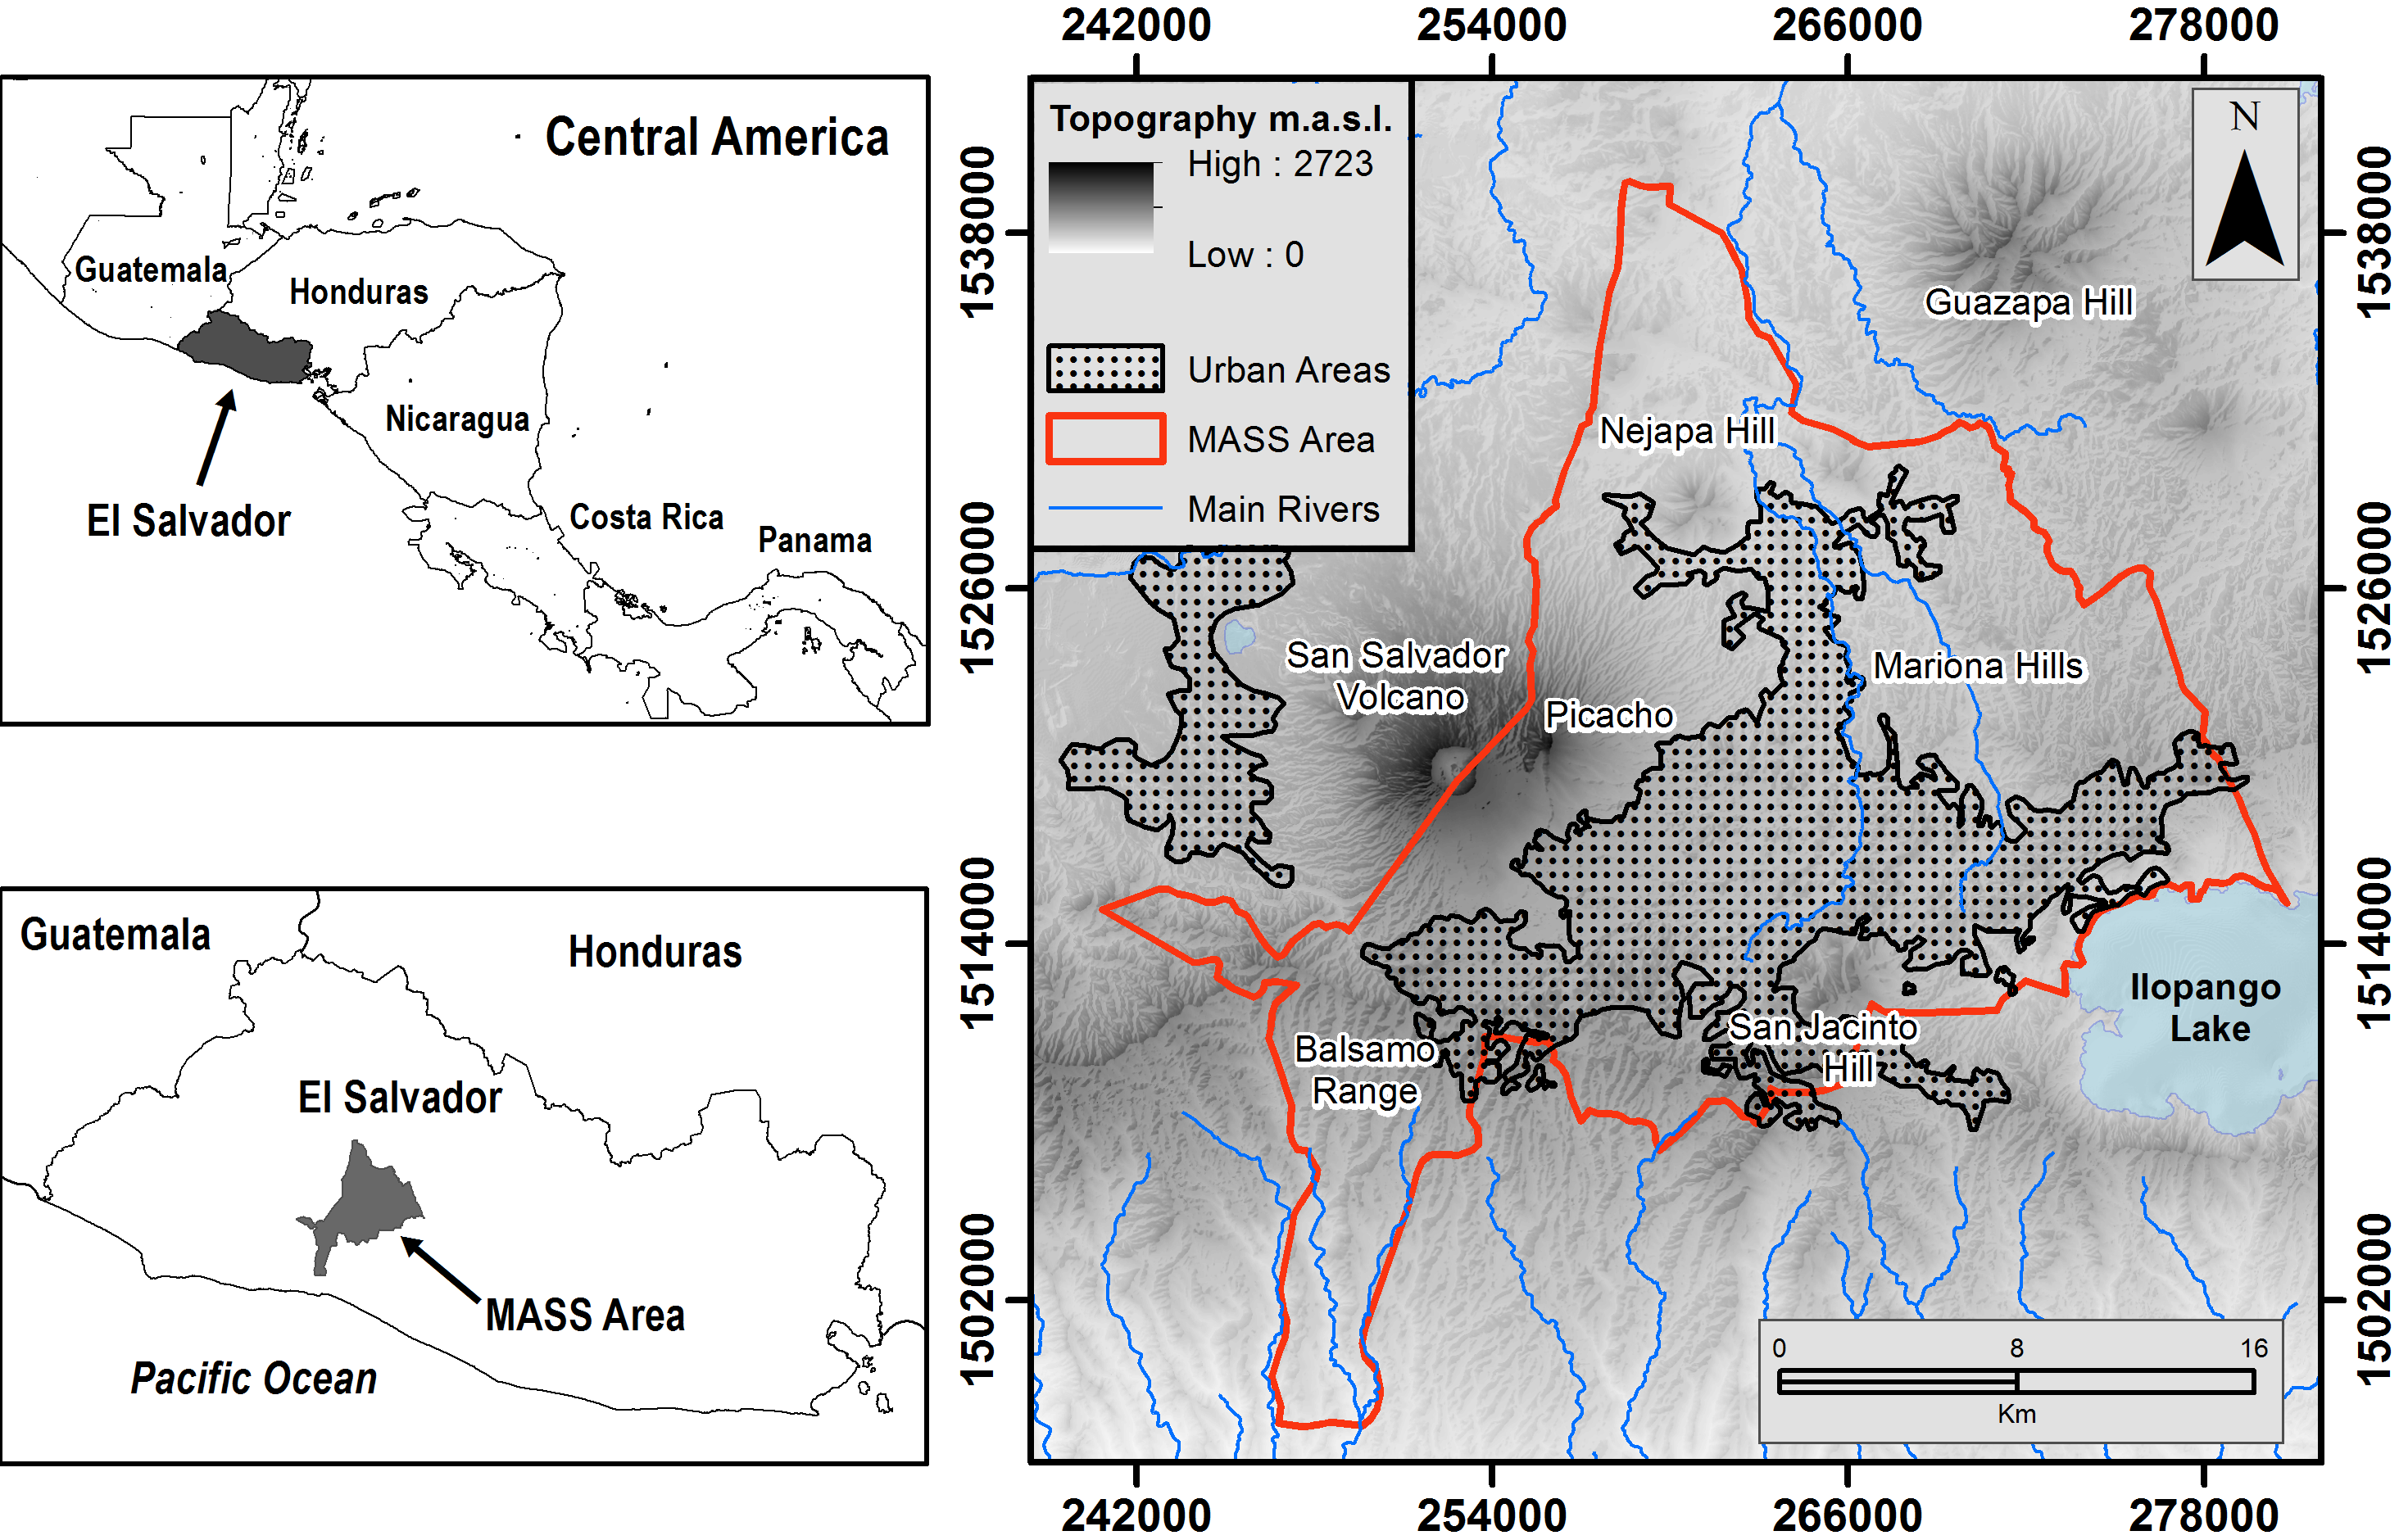
\includegraphics[scale=0.70]{MASS_mapa_1}
   \caption{\small{Location of El Salvador in Central America, map of El Salvador with location of the Metropolitan Area of San Salvador (MASS) and its topography.}}
   \label{fig:mass01}
  \end{figure}
 \end{center}




\section{Brief State of Art}
\label{sec:brief}
Since the pioneering work \cite{Carrara1983403}, several mathematics and statistics models have been proposed to model landslide susceptibility: deterministic models (\cite{hessd-10-12643-2013},  \cite{doi:10.1080/19475705.2010.498151} and \cite{Neu2012511}), probabilistic models (\cite{Bern198839}, \cite{Chung2003451} and \cite{doi:10.1080/01431160310001618734} ). 

It has been used popular classification models such as logistic regression (\cite{akgun2012} and \cite{gaskill} and \cite{garcia2008} ) , neural networks (\cite{garcia2010}, \cite{Melchiorre2011410},\cite{Zeng2001374}, \cite{Ermini2005327} and \cite{Yesilnacar2005251})  and support vector machine (\cite{ballabio2012support} and \cite{tien2012landslide}). 


According to \cite{van2006landslide} the magnitude of a possible
slide is difficult to foresee as it depends on the magnitude of the triggering event and the environmental conditions (e.g., height of water table) at the moment of the event. Because of these complex relationships between the dependent variable and causal factors, and since that neural networks are particularly useful for detect complex non-linear relationships in large datasets, that is why this kind of model was chosen, despite the disadvantages such as greater computational burden and proneness to overfitting.  



\section{Study area}
\label{sec:studyarea}
MASS, is formed by 14 municipalities among them it is located San Salvador, the capital of the country. It has 587 $km^{2}$ and according to the most recent census \cite{minecon} it has 1,566,629 inhabitans with a density of population of 2669 hab/km2.  According to geography MASS is extended over a flat erosional surface (650-760 m.a.s.l.), gently sloping to the east towards Ilopango Caldera also known as Ilopango Lake. MASS is bordered to the south by the Balsamo Range and San Jacinto Hill, to the west by San Salvador volcano and with Mariona Hills (refer to Fig. \ref{fig:mass01}). Human settlement is not only restricted to the plain, but spreads up to surrounding heights and volcano flanks.

All rocks exposed in MASS have volcanic origin and consists of intercaled primary and reworked deposits from Late Tertiary to Holocene age \cite{schmidt1975}. The younger ones are known as Tierra Blanca pyroclastic ash deposits and forms a relative continuous layer in majority of MASS with an average thickness of 4 m \cite{schmidt1975}. These are deposits derived mainly from Ilopango caldera eruptions where they present more than 50 m of thickness \cite{schmidt1975}. Tierra Blanca soils is highly susceptible to erosion, one of the most common dangerous effects of the erosion in this area are landslides during heavy rainfall and earthquake ground shaking \cite{schmidt1975}. Ch\'{a}vez et al. \cite{chavez2014a} identified high and moderate erosion hazard in majority of MASS area. The more recent layer Tierra Blanca, known as Tierra Blanca Joven (TBJ) \cite{hernan2004} present very poor geotechnical properties, especially when there is an increment of soil moisture (i.e. during rainy seasons), which results in high instability susceptibility (\cite{chavez2014b} and \cite{rolo2004}). Several incised rivers and ravines cross MASS area, due the large erosion rates of the area, natural slopes of these watercourses are often close to vertical and can reach highs of more than 10 m. Taking into account this property of volcanic soils, usually vertical slopes are cut to urban and road construction. As Bommer \& Rodriguez \cite{bommer} identified in Central America, although such slopes may remain stable for years, they may become unstable, abruptly and totally under the action of heavy rainfall or seismic shaking. Hern\'{a}ndez \cite{hernan2004} carried out a detailed description of this process in TBJ, where these instabilities are very common. 
In study area fault trends are characterized by steep dip angles (65\textdegree - 90\textdegree). The main fault system is characterized by an east-west trend; this trend is responsible of the steep northern slope of the El Balsamo Range.  The secondary systems are with north, northwest and northeast trends offset the main fault system and are more active in the present tectonic setting \cite{schmidt1975}. However, all the mentioned fault families appear active. Thus the several fault systems have developed at different times, but been repeatedly activated \cite{rymer1987}. Finally there are also several ringlike faults that can be related to subsurface collapse due to volcanic tectonic subsidence \cite{schmidt1975}.
Last eruption of San Salvador volcano was 1917.  The majority of the magma's total volume (97\%) extruded from several vents in the Northwest flank of the volcano, outside of MASS. However a fraction of MASS is located under the proximal volcanic hazard zone according to Sofield \cite{sofield2004}. In the steep slopes  San Salvador volcano, especially of Picacho, the highest peak of the volcano, located in the eastern side present a high lahar hazard that threats MASS \cite{major2004}. On the other hand one of the most destructive eruptions in the world history was 430 A.D. TBJ eruption produced by the Ilopango Caldera. According to Dull \cite{dull2004}, that eruption produced total devastation in whole MASS area. 




\section{Landslide inventory and data sources of input variables}
\label{sec:landsinvet}
The Landslide inventory was developed by MARN and it was conducted in two stages. The first was carried out, based on fieldwork after the 2001 earthquakes in El Salvador. The second stage consisted of a visual inventory of places where there were landslides identified through satellite image from IRS-C sensor (Indian) in the same year.


Once the landslide inventory was finished, a percentage of 0.5\% of the total points georeferenced showed landslide occurrence. In addition to the landslide information the following data sources of input variables was provided by MARN: 


\begin{enumerate}
\item {\bf Geomorphology:} refers to landforms that result from lithospheric dynamics of geographic area. This variable was obtained in the project of national land use plan in El Salvador. It is unpublished geomorphologic cartography in digital format provided by MARN.


\item {\bf Slope:} Slope gradient is an important component and a
preparatory cause of landsliding \cite{garcia2008}. It was calculated from digital elevation model (DEM) provided by MARN with a resolution of 10 mt. 

\item {\bf Geology:} Description of the geology of the area according digitalized geological map of  El Salvador (scale 1:100,000) \cite{weber}.

\item {\bf Rainfall intensity:} From the precipitation database compiled by the
MARN's weather stations for the period 1970–2001, maximum precipitations were obtained, 
and then, a contour map was generated through kriging interpolation method.

\item {\bf Peak ground accelaration:} Maximum ground acceleration expressed in Gal for a return period of 500 years. This data was obtained from the evaluation of seismic Hazard in Central America carried out under the framework of RSIS II project \cite{beni2012}.

\item {\bf Road distance:} Distance in kilometers to the nearest road. Road map was obtained from digitalized national cartography created by Centro Nacional de Registros de la Rep\'{u}blica de El Salvador (CNR).

\item {\bf Fault distance:} Distance in kilometers to the nearest fault. This information was obtained from according digitalized geological map of El Salvador (scale 1:100,000) \cite{weber}.
 
\end{enumerate}



\section{Artificial Neural Network model for discrete choice}
Logistic regression represents a neural network with 
a neuron in the hidden layer and whose output is dichotomous. The following adapted form of the Multilayer Perceptron (MLP) may be used for modeling binary classification problems. In the equation (\ref{eq:ann1}) $x_{k,i}$ are the observed values in the ith input variables belonging to the kth case. The expressions $w_{j,k}$ and $\lambda_{j}$ showed in the equations (\ref{eq:ann1}) and (\ref{eq:ann3}) are the parameters of the model. 


\begin{equation}
n_{j,i} = w_{j,0} + \sum_{k=1}^{k^{*}} w_{j,k}x_{k,i}
\label{eq:ann1}
\end{equation}

\begin{equation}
N_{j,i} = \frac{1}{1+\exp^{-n_{j,i}}}
\label{eq:ann2}
\end{equation}



\begin{equation}
p_{i} = \sum_{j=1}^{j^{*}} \lambda_{j} N_{j,i}
\label{eq:ann3}
\end{equation}

\begin{equation}
\sum_{j=1}^{j^{*}} \lambda_{j} = 1 , \lambda_{j} \ge 0
\label{eq:ann4}
\end{equation}


In the equation (\ref{eq:ann3}) $p_{i}$ is the the predicting probability for a network with $ k^{*} $ input characteristics and $ j^{*} $ neurons. In the context of the present research, $p_{i} $ represents the probability of landslide ocurrence.

Before estimating the parameters of the neural network model, it is necessary standardize the input variables. In particular for classification problems is more suitable to scale inputs to $[-1,1]$ rather than $[0,1]$ \cite{FAQANN}. The following scaling was applied to each input variable: 

\begin{equation}
z = \frac{x - \bar{x} }{\sigma_{x}}
\label{eq:scaling}
\end{equation}

In the equation (\ref{eq:scaling}) $z$ is the new variable transformed, $ \bar{x} $ and $\sigma_{x}$ are, respectively the mean and the standard deviation of the input variable to transform.  

The method used for estimating the parameters of the model was an Hybrid Method \cite{McNelis2005}. Firstly heuristic genetic algorithm using a package developed in the R statistical software \cite{rproject} specifically developed for this purpose, was used to obtain a good estimation of the parameters of the model. 

The R package can be accessed from the following web address:
 
\url{https://goo.gl/PHaaG2}


Once a good estimate was obtained, this was occupied as the initial values for the conjugate gradient method implemented in the optim routine of the R statistical software, to obtain a better estimation of the parameters of the model.  


\section{Spatial Prediction}

\subsection*{Estimating spatial correlation}

In standard statistical problems, correlation can be estimated from a scatterplot, when several data pairs ${x, y}$ are available. The spatial correlation between two observations of a variable $z(s)$ at locations $s_{1}$ and $s_{2}$ cannot be estimated, as only a single pair is available. To estimate spatial correlation
from observational data, it is necessary to make stationarity assumptions
before we can make any progress. One commonly used form of stationarity
is intrinsic stationarity, which assumes that the process that generated the
samples is a random function $Z(s)$ composed of a mean and residual \cite{bivand2008applied}:

\begin{equation}
Z(s) = \mu + \delta(s)
\end{equation}

with a constant mean 

\begin{equation}
E\left(Z(s)\right) = \mu
\end{equation}

and a variogram defined as 

\begin{equation}
\lambda(h) = \frac{1}{2}E\left(Z(s) - Z(s+h)\right)^{2}
\end{equation}


\subsection*{Ordinary kriging in terms of the covariance function}
The predictor assumption is 
\begin{equation}
\hat{Z(s_{0})} = \sum_{i=1}^{n} w_{i}Z(s_{i})
\end{equation}

It is a weighted average of the sample values, and $ \sum_{i=1}^{n} w_{i} = 1 $ to ensure unbiasedness. The $w_{i}$'s are the weights that will be estimated. Kriging minimizes the mean squared error of prediction \cite{nicolas2015}. 

\begin{equation}
min \ \sigma_{e}^{2} = E\left[Z(s_{0}) - \hat{Z(s_{0})}\right]^{2}
\end{equation}  



\section{Results}
The data were randomly divided into three sub-samples, the first was used for the
estimation of the parameters of the neural network model (training set), the second was used to choose the model with more generalization capability (validation set) and the last was
used to evaluate how well the model generalize outside of the data set used for estimation (test set). 

To determine the number of neurons in the hidden layer, the method of trial and error was used, starting with few neurons and increasing progressively the number of neurons in the hidden layer. Table \ref{annresults}
summarizes how well the models fit on the training, validation and test sets.

\begin{table}[H]
\caption{Summary of classification accuracy on the training, validation and test sets for neural network models  }
\label{annresults}
\centering
\begin{tabular}{ | c | c | c | c | }
\hline
\multicolumn{4}{| c |}{Percentage score} \\
\hline
Number of neurons &    Train set    &   Validation set &  Test set \\
\hline
2  &  0.7011 & 0.7020 & 0.7124 \\
\hline
3 &  0.7206 & 0.7072 & 0.7401 \\
\hline 
4 &  0.7425 & 0.7197 & 0.7458 \\
\hline
5 &  0.7601 & 0.7604 & 0.7740 \\
\hline
6 &  0.7823 & 0.7704 & 0.7604 \\
\hline
7 &  0.7853  & 0.7704 &  0.7763 \\
\hline
8 &  0.7942 & 0.7865 & 0.7878  \\
\hline
9 & 0.8009 & 0.7871 & 0.7901  \\
\hline
10 & 0.8321 & 0.8132 & 0.8009  \\
\hline
11 & 0.8194 & 0.7792 & 0.7542 \\
\hline
12  &  0.8230 & 0.8006 & 0.8159 \\
\hline
13 & 0.8408 &  0.8006 & 0.8031 \\
\hline
14  &  0.8373 & 0.8017 & 0.8127 \\
\hline
15 &  0.8517 & 0.8210 & 0.8247 \\ 
\hline
16  &  0.8246 & 0.8017 & 0.8028 \\ 
\hline
17  &  0.8543 & 0.8283 & 0.8246 \\ 
\hline
18   &  0.8467 & 0.8022 & 0.8418 \\ 
\hline
19  &  0.8341  & 0.7991 & 0.8274 \\
\hline
\end{tabular}
\end{table}


The model with 17 neurons in the hidden layer was chosen because it presents the best performance in the validation set. After that a logistic regression model was fitted as a basis of comparison. In the Table \ref{logisticresults} is presented logistic regression model results. Clearly, neural network model chosen has better performance than logistic regression model.

\begin{table}[H]
\caption{Summary of classification accuracy on the training, validation and test sets for logistic regression}
\label{logisticresults}
\centering
\begin{tabular}{ | c | c | c | c | }
\hline
\multicolumn{4}{| c |}{Percentage score} \\
\hline
Model &    Train set    &   Validation set &  Test set \\
\hline
logistic regression  &  0.6710  & 0.6748   & 0.663 \\
\hline
\end{tabular}
\end{table}
 
To generate the map of landslide hazards, the following steps were followed based on geostatistics methodology: Exploratory analysis, Variogram modelling and Spatial prediction using ordinary kriging, validation, and exporting the spatial predictions to raster format. 

In order to achieve the above steps, an R script was developed. This script can be downloaded in:

\url{https://goo.gl/3N8n99}

First of all one thousand fifty georeferenced points with their probability of occurrence calculated using neural network, were selected randomly for the map generation process leaving the others for validation of the kriging model. The Exploratory analysis showed the presence of spatial correlation, this was done making scatter plot of pairs $Z(s_{i})$ and  $Z(s_{j})$, grouped according to their separation distance, also the data did not show the presence of anisotropic effect. 

Regarding variogram estimation the spherical, gaussian and exponential models were proposed. The validation of these models on data were not taken into account in the process of estimating the variogram showed that the best model was the exponential, since it had an $ R^{2} = 0.42 $ against $ R^{2} = 0.40 $ and $ R^{2} = 0.39 $ of the models spherical and gaussian respectively. Using exponential model, spatial predictions were calculated on a grid of 1500 $\times$ 1500 and exported to Geotiff raster format. Finally Geographic Information System (ArcGIS\textregistered \  of ESRI) was used to design the final map (Figure \ref{fig:mass02}). This map (Fig. \ref{fig:mass02}) represents the landslide probability of occurrences in MASS. According to Fig. \ref{fig:mass02} higher probability of landslide occurrence are around 0.8, and are located in the northern slopes of Balsamo Range (western side of MASS), in the eastern slope of San Salvador volcano and Picacho,  along the extension of Mariona Hills  and in the southeastern side, between Ilopango lake and San Jacinto Hill. Areas with lower probability but still important, are located in southern and western side of Nejapa Hill, in north-east of the study area, in northern banks of Ilopango lake, in northeast slope of San Salvador Volcano, in the surrounding areas of San Jacinto Hill and, in general in southern side of MASS. 





\section{Discussion and conclusions}
A landslide hazard assessment study was carried out in Metropolitan Area of San Salvador (MASS). The study started with the construction of a landslide inventory and analysis of the causal factors related to the occurrences of landslide. The problem of modeling landslide is very complex and for this reason the study proved the efficacy of the neural network model with a percentage of correct classification around 80\% against other models such as logistic regression with a percentage of correct classification under 70\%. 

In the process of estimating the weights of the model, an heuristic technique was used to obtain a better solution after that a local search was used. The difficulty of this approach is due to intensive computation involved in the estimation of a neural network model takes between 4 and 10 hours. For this reason the statistical significance of the input variables could not be assessed by means boostrapping  (a statistical resampling technique). For all of the above parallel computing must be used rather than serial computing to estimate weights of a neural networks models.



The results obtained through geostatistical methodology met the assumptions for kriging method application. Final map of landslide probability of occurrence (see Fig. \ref{fig:mass02} ) generated by kriging method was the result of multidisciplinary work which implied an intense geological analysis (i.e. MARN inventory of 4792 landslides) together with the use of sophisticated statistical techniques. This landslide hazard map is a user-friendly tool to evaluate landslide risk in MASS and can be useful for many purposes such as territorial planning, prevention and landslide mitigation and so on. 
\begin{center}
  \begin{figure}
   \centering
   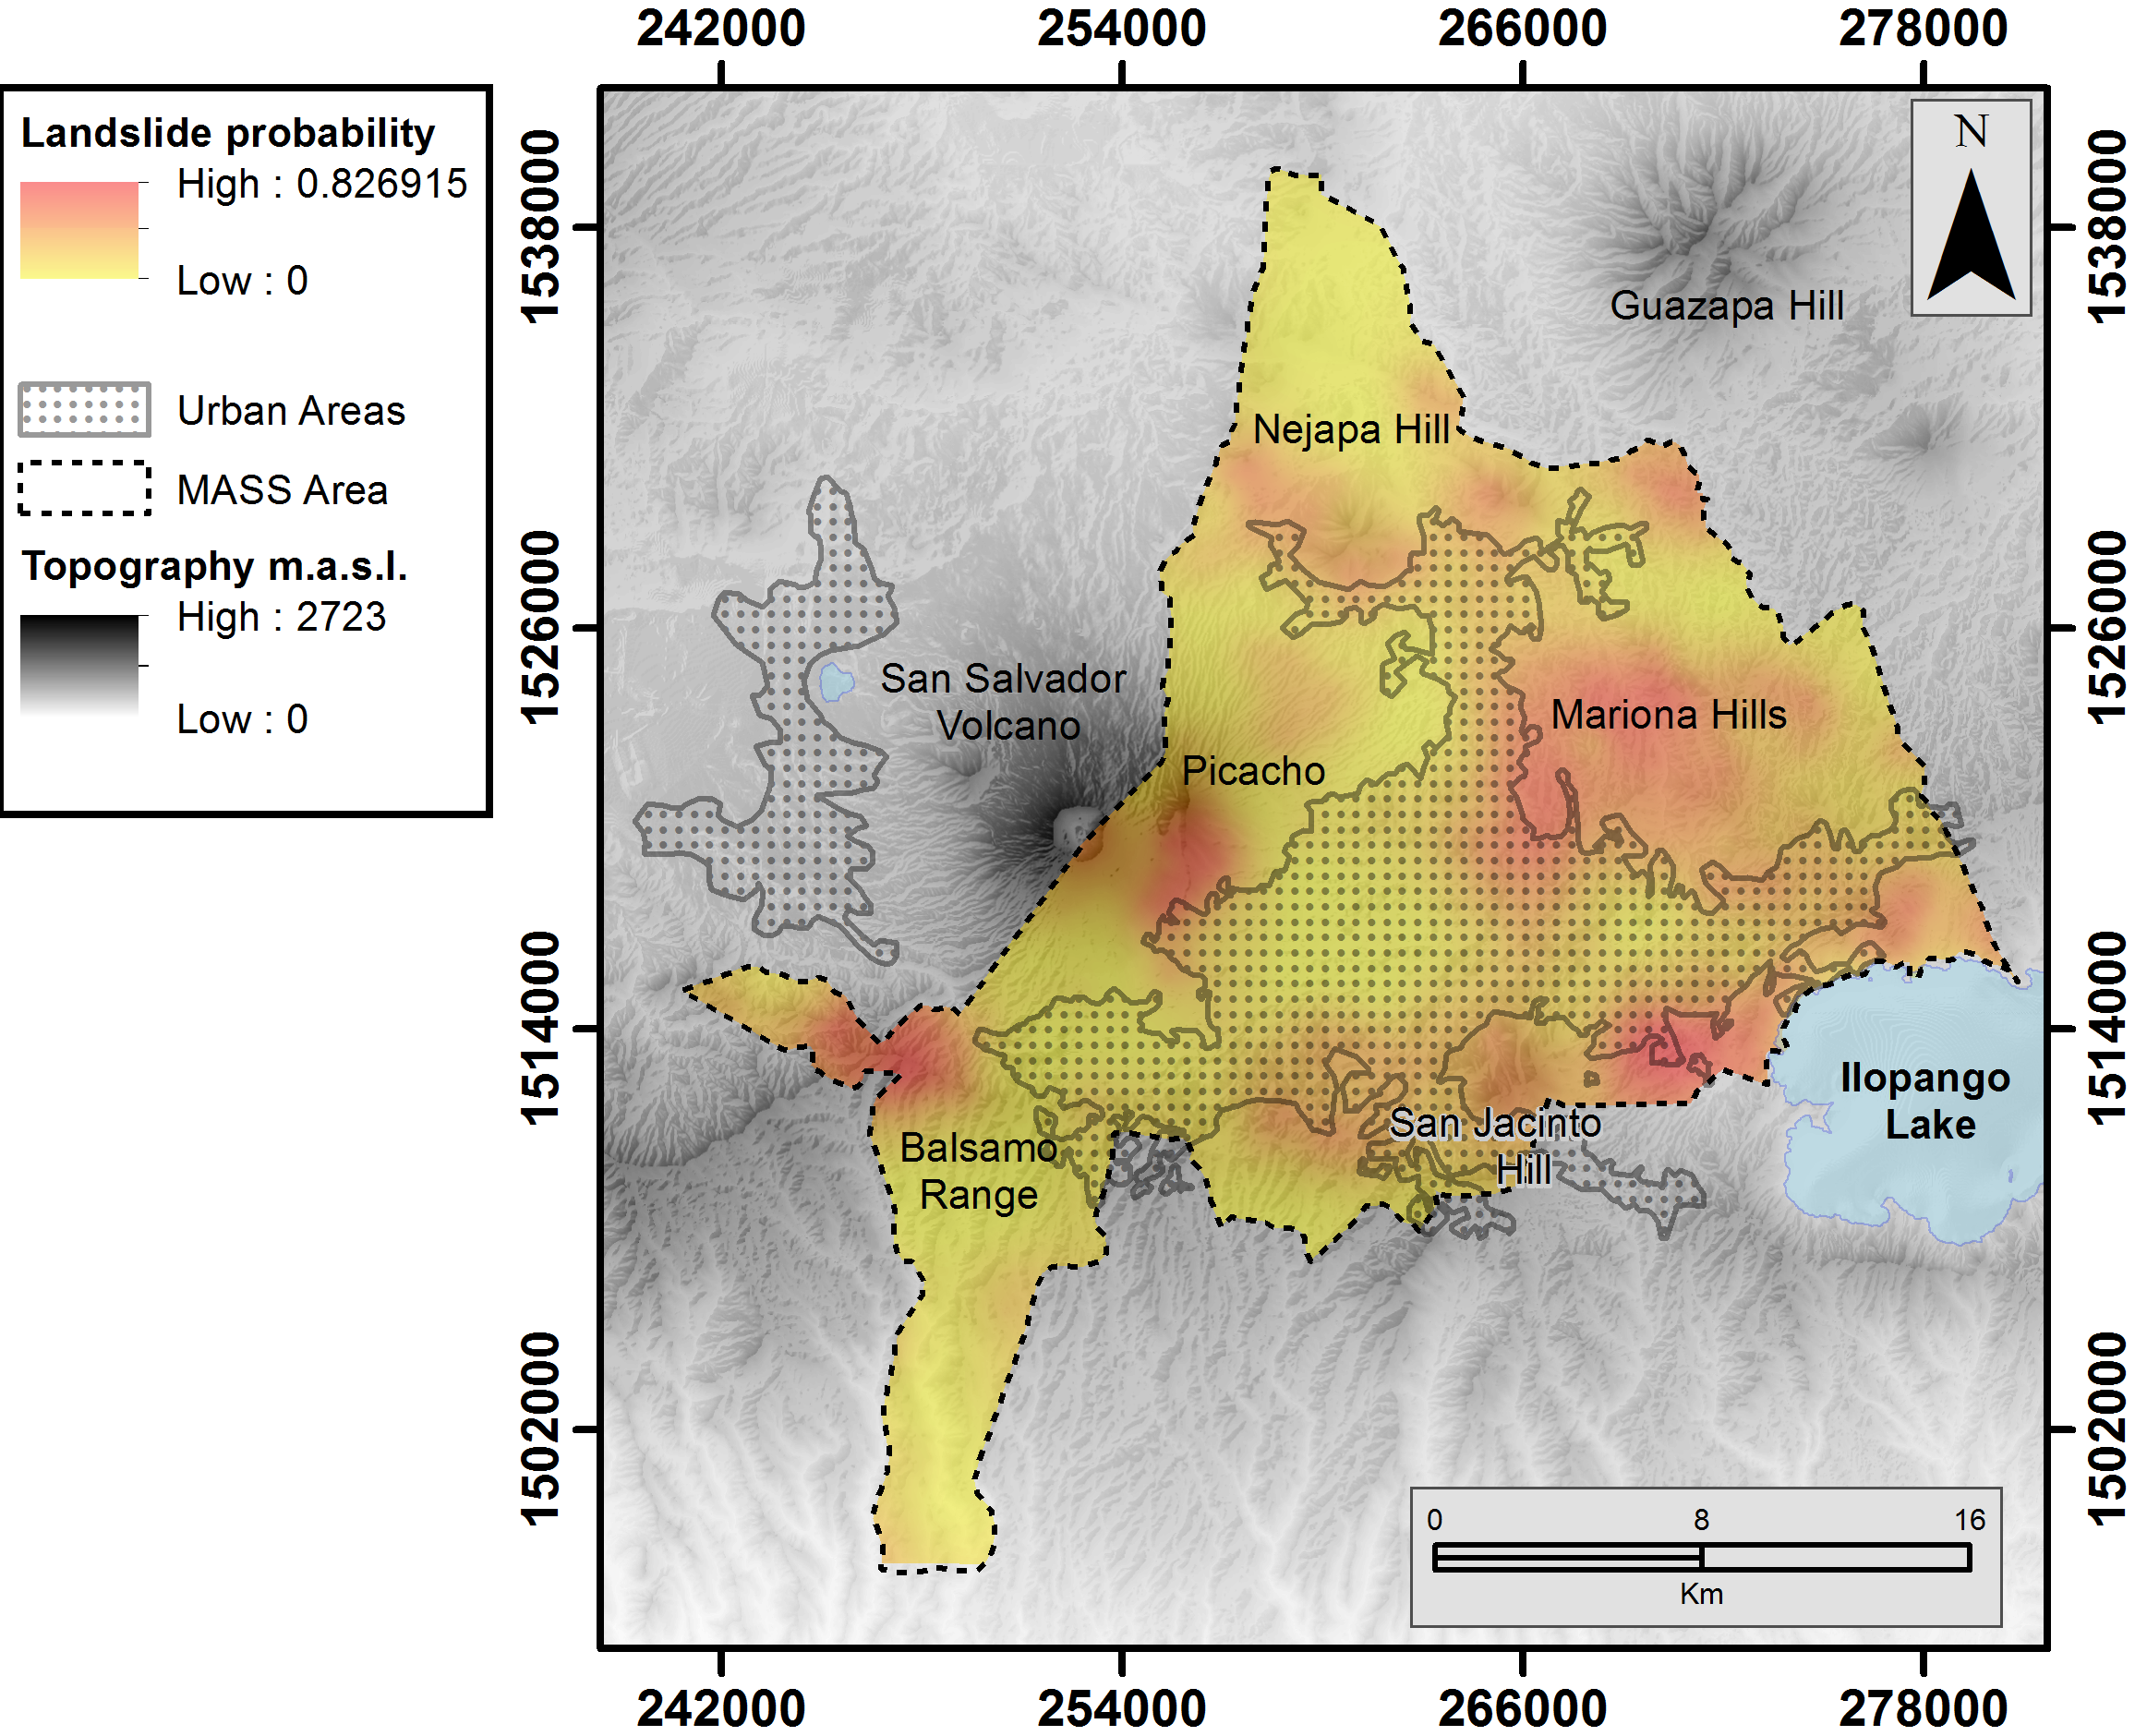
\includegraphics[scale=0.73]{MASS_mapa_2}
   \caption{\small{Landslide hazard map MASS where the landslide probability of occurrence is shown.}}
   \label{fig:mass02}
  \end{figure}
 \end{center}
High probability of landslide occurrence in Picacho slope implies very high risk due the proximity of urban areas and due the large volume of mobilized materials. Major et al.\cite{major2004} identified in San Salvador volcano lahars as voluminous as 2 million of $mts^{3}$ that can affect large zones of urban areas. Southern areas of MASS also implies a high risk because landslides, similar to Las Colinas landslide which involved a total volume of around 200,000 m3 \cite{evans}, can occur in northern slope of Balsamo range and San Jacinto Hill affecting very crowded urban areas.

The present hazard landslide map is consistent with former landslide hazard maps carried out in the region using approaches conceptually different. Fern\'{a}ndez-Lavado et al.\cite{fernan2008} presented a landslide hazard GIS map of MASS generated through bivariate statistical method considering several conditioning factors showing similar hazard areas. The only differences are located mainly in the Nejapa Hill, San Jacinto Hill where Fern\'{a}ndez-Lavado et al. \cite{fernan2008} identified a slightly higher hazard and the area between San Jacinto Hill and Ilopango Lake where the former study presented a hazard slightly lower. As landslides are an erosional phenomenon, the highest probability areas of landslide occurrence coincides with the areas with highest hazard of erosion in the erosion hazard map of MASS proposed by Ch\'{a}vez et al. \cite{chavez2014a}. There are similarities with susceptibility hazard maps at national scale generated through logistic regression method \cite{garcia2008}, through artificial neural network method \cite{garcia2010} and through Mora-Vahrson method \cite{snet2004}. However the high landslide areas are more extended in these national maps than the present study. These differences could be explained by the working scale, our map is more detailed because is at regional scale. Other possible explanation can be related to the data, present work was built using a more extended landslide catalog and more updated data (e.g. seismic hazard evaluation from Benito et al. cite{beni2012} than former works.

Rock falls were not included in the catalog; these were very common during 2001 earthquakes in El Balsamo Range \cite{jibson}. On the other hand, the MASS seismic microzonation of seismic site effects will improve the estimation of peak ground acceleration. The local geologic conditions are responsible for the modifications (amplification, frequency content and duration) experimented by seismic motions just before reaching the ground surface, additionally, the geometry of the ground surface also may produce amplification (topographic effects) \cite{aki1993}. These effects can be important in soft soils close to incised rivers and also in San Salvador volcano, Balsamo ranges and hills. Crosta et al. \cite{crosta2005} identified an amplification factor of 1.3-1.4 in the Las Colinas failure area (Balsamo Ranges). All these variables can improve the predictive ability of the model and surely the likelihood of landslides.



\section{Acknowledgment}   
The authors are indebted with MARN who provided the data and Geographic Information System software such as ILWIS and ArcGIS\textregistered \  of ESRI.



\begin{thebibliography}{99}




\bibitem{dewey}
Dewey J.W. White R.A., Hern\'{a}ndez D.A.
\newblock Seismicity and tectonics of El Salvador
\newblock \emph{Chapter 27 in Geological Society of America Special paper 375 in Natural Hazards in El Salvador of Rose W.I., Bommer J.J., L\'{o}pez D.L., Carr M.J. and Major J.J. 367-378. (2004)}


\bibitem{weber}
Weber H.S., Wiesemann G., Lorenz  W., Schmidt-Thom\'{e} M.
\newblock Mapa geol\'{o}gico de Republica de El Salvador
\newblock escala 1 : 100 000 (6 sheets).
\newblock \emph{ Bundesanstalt f\"ur Geowissenschaften und Rohstoffe, Hannover, Germany.
}
\penalty0 (1978).


\bibitem{bommer}
Bommer J.J., Rodriguez C.E.
\newblock Earthquake-induced landslides in Central Am\'{e}rica
\newblock \emph{Engineering Geology}.
(63):\penalty0 1889-220, (2002).


\bibitem{evans}
Evans S.G. Bent A.L.
\newblock Las Colinas landslide, Santa Tecla:  A higly destructive flowslide triggered by January 13, 2001, El Salvador earthquake.
\newblock \emph{Chapter 3 in Geological Society of America Special paper 375 in Natural Hazards in El Salvador of Rose W.I., Bommer J.J., L\'{o}pez D.L., Carr M.J. and Major J.J. 25-37. (2004)}



\bibitem{jibson}
Jibson R.W., Crone A.J., Harp E.L., Baum R.L., Major J.J., Pullinguer C.R., Escobar D., Martinez M., Smith M.E. 
\newblock Landslides triggered by the 13 January and 13 February 2001, earthquakes.
\newblock \emph{ Chapter 6 in Geological Society of America Special paper 375 in Natural Hazards in El Salvador of Rose W.I., Bommer J.J., L\'{o}pez D.L., Carr M.J. and Major J.J. 69-88. (2004)}



\bibitem{crone}
Crone A.J., Baum R.L., Lidke D.J., Sather D.N.D., Bradley L.-A., Tarr A.C.
\newblock Landslides Induced by Hurricane Mitch in El Salvador-An Inventory and Description of Selected Features
\newblock \emph{USGS Open File Repord 01-444. (2002)}


\bibitem{Carrara1983403}
Alberto Carrara.
\newblock Multivariate models for landslide hazard evaluation.
\newblock \emph{Journal of the International Association for Mathematical
  Geology.}, 15\penalty0 (3):\penalty0 403--426, 1983.
\newblock ISSN 0020-5958.


\bibitem{hessd-10-12643-2013}
G.~Capparelli and P.~P.~Versace.
\newblock Landslide susceptibility from mathematical model in sarno area.
\newblock \emph{Hydrology and Earth System Sciences Discussions}, 10\penalty0
  (10):\penalty0 12643--12662, 2013.


\bibitem{doi:10.1080/19475705.2010.498151}
Biswajeet Pradhan, Hyun-Joo Oh, and Manfred Buchroithner.
\newblock Weights-of-evidence model applied to landslide susceptibility mapping
  in a tropical hilly area.
\newblock \emph{Geomatics, Natural Hazards and Risk}, 1\penalty0 (3):\penalty0
  199--223, 2010.
  
  
\bibitem{Neu2012511}
Bettina Neuh\"auser, Bodo Damm, and Birgit Terhorst.
\newblock Gis-based assessment of landslide susceptibility on the base of the
  weights-of-evidence model.
\newblock \emph{Landslides}, 9\penalty0 (4):\penalty0 511--528, 2012.
\newblock ISSN 1612-510X.


\bibitem{Bern198839}
Campbell R.H. Brookshire~D.S. Bernknopf, R.L. and C.D Shapiro.
\newblock A probabilistic approach to landslide hazard mapping in cincinnati,
  ohio, with application for economic evaluation.
\newblock \emph{Bulletin of the Association of Engineering Geologists},
  XXV\penalty0 (1):\penalty0 39--56, 1988.
  
  
\bibitem{Chung2003451}
Chang-JoF. Chung and AndreaG. Fabbri.
\newblock Validation of spatial prediction models for landslide hazard mapping.
\newblock \emph{Natural Hazards}, 30\penalty0 (3):\penalty0 451--472, 2003.
\newblock ISSN 0921-030X.
\newblock doi:{10.1023/B:NHAZ.0000007172.62651.2b}.

\bibitem{doi:10.1080/01431160310001618734}
S.~Lee, J.~Choi, and K.~Min.
\newblock Probabilistic landslide hazard mapping using gis and remote sensing
  data at boun, korea.
\newblock \emph{International Journal of Remote Sensing}, 25\penalty0
  (11):\penalty0 2037--2052, 2004.
  
  
  
\bibitem{akgun2012}
Akgun, Aykut
\newblock A comparison of landslide susceptibility maps produced by logistic regression, multi criteria decision, and likelihood ratio methods: a case study at Izmir, Turkey
\newblock \emph{Landslides},
  (11):\penalty0 9, 1, 93--106, 2012.
\newblock Springer. 


\bibitem{gaskill}
Gaskill, Jacob and Zuber, Brian and Nordman, Erik
\newblock Analyzing Landslide Susceptibility in St. Vincent and the Grenadines Using Co-Kriging and Logistic Regression
\newblock \emph{The 2015 IMAGIN Award, Michigan United States}.

  
\bibitem{garcia2008}
Garc\'{i}a-Rodr\'{i}guez M.J., Malpica J.A., Benito B., D\'{i}az M.
\newblock  Susceptibility assessment of earthquake-triggered landslides in El Salvador using logistic regression.
\newblock \emph{Geomorphology}
\penalty0 95, 172-191, 2008. 
  


\bibitem{garcia2010}
Garc\'{i}a-Rodr\'{i}guez M.J., Malpica J.A.
\newblock Assessment of earthquake-triggered landslide susceptibility in El Salvador based on an Artificial Neural Network model.
\newblock \emph{Nat. Hazards Earth Syst. Sci.}
\penalty0 10, 1307–1315, 2010. 
\newblock doi:10.5194/nhess-10-1307-2010.
  

\bibitem{Melchiorre2011410}
C.~Melchiorre, E.A.~Castellanos Abella, C.J. van Westen, and M.~Matteucci.
\newblock Evaluation of prediction capability, robustness, and sensitivity in
  non-linear landslide susceptibility models, guant\'{a}namo, cuba.
\newblock \emph{Computers {\&} Geosciences}, 37\penalty0 (4):\penalty0 410 --
  425, 2011.
\newblock ISSN 0098-3004.


\bibitem{Zeng2001374}
Xu~Zeng-wang.
\newblock Gis and ann model for landslide susceptibility mapping.
\newblock \emph{Journal of Geographical Sciences}, 11\penalty0 (3):\penalty0
  374--381, 2001.
\newblock ISSN 1009-637X.
\newblock doi:{10.1007/BF02892323}.


\bibitem{Ermini2005327}
Artificial neural networks applied to landslide susceptibility assessment.
\newblock \emph{Geomorphology}, 66\penalty0 (1–4):\penalty0 327 -- 343, 2005.
\newblock ISSN 0169-555X
\newblock doi:10.1016/j.geomorph.2004.09.025.



\bibitem{Yesilnacar2005251}
E. Yesilnacar and T. Topal.
\newblock Landslide susceptibility mapping: A comparison of logistic regression and neural networks methods in a medium scale study, Hendek region (Turkey).
\newblock \emph{Engineering Geology}, 79\penalty0
  (11):\penalty0 251-266, 2005.
\newblock ISSN 0013-7952,
\newblock doi:10.1080/01431160310001618734.




\bibitem{ballabio2012support}
Ballabio, Cristiano and Sterlacchini, Simone
\newblock Support vector machines for landslide susceptibility mapping: the Staffora River Basin case study, Italy
\newblock \emph{Mathematical geosciences},
  (11):\penalty0 1, 47--70, 2012.
\newblock Springer. 



\bibitem{tien2012landslide}
Tien Bui, Dieu and Pradhan, Biswajeet and Lofman, Owe and Revhaug, Inge
\newblock Landslide susceptibility assessment in vietnam using support vector machines, decision tree, and Naive Bayes Models
\newblock \emph{Mathematical Problems in Engineering},
  (11):\penalty0 2012, 2012.
\newblock Hindawi Publishing Corporation.




\bibitem{van2006landslide}
Van Westen, CJ and Van Asch, Th WJ and Soeters, R
\newblock Landslide hazard and risk zonation why is it still so difficult?
\newblock \emph{Bulletin of Engineering geology and the Environment}.
(65):\penalty0 2, 167--184, 2006
\newblock Springer. 



\bibitem{minecon}
Ministerio de Economia- Direcci\'{o}n General de Estad\'{i}stica y Censos
\newblock VI Censo de Poblaci\'{o}n y V de Vivienda
\newblock \emph{2007-2008}.
\penalty0 Available from http://goo.gl/yvjzPy




\bibitem{schmidt1975}
Schmidt-Thom\'{e} M.
\newblock The geology in San Salvador area (El Salvador, Central America), a basis for city development and planning.
\newblock \emph{Geol. Jb.}.
\penalty0 13, 207-228, 1975.


\bibitem{chavez2014a}
Ch\'{a}vez J.A., Sebesta J., Kopecky L., L\'{o}pez R.
\newblock Application of Geomorphologic Knowledge for Erosion Hazard Mapping
\newblock \emph{Natural Hazards}.
\penalty0 71,1323–1354, 2014.
\newblock doi:10.1007/s11069-013-0948-8.


\bibitem{hernan2004}
Hern\'{a}ndez W.E.
\newblock Caracter\'{i}sticas Geomec\'{a}nicas y Vulcanologicas de las Tefras Tierra Blanca Joven, Caldera de Ilopango, El Salvador.
\newblock MSc Thesis. Universidad Polit\'{e}cnica de Madrid – Universidad Polit\'{e}cnica de El Salvador.
\penalty0 2004


\bibitem{chavez2014b}
Ch\'{a}vez J.A.,  Landaverde J.M., Ayala O.E., Mendoza L.E. (2014b). 
\newblock Application of Constitutive Models in the Volcanic Tephra ``Tierra Blanca Joven''.
\newblock \emph{Ingenier\'{i}a.}
\penalty0  24 (2).53-78.
\newblock  ISSN: 2215-2652.


\bibitem{rolo2004}
Rolo R., Bommer J.J., Houghton B.F., Vallance J.W., Berdousis P., Mavrommati C., Morphy W.
\newblock Geologic and engineering characterization of Tierra Blanca pyroclastic ash deposits.
\newblock \emph{Chapter 5 in Geological Society of America Special paper 375 in Natural Hazards in El Salvador of Rose W.I., Bommer J.J., L\'{o}pez D.L., Carr M.J. and Major J.J.}
\penalty0  55-67, 2004.


\bibitem{rymer1987}
Rymer M.J. 
\newblock The San Salvador Earthquake of October 10, 1986.
\newblock \emph{Geologic Aspects Earthquake Spectra.}
\penalty0 3(3), 435-463, 1987.


\bibitem{dull2004}
Dull R.A.
\newblock Lessons from the mud, lessons from the Maya: Paleoecological records of the Tierra Blanca Joven eruption.
\newblock \emph{Chapter 7 in Geological Society of America Special paper 375 in Natural Hazards in El Salvador of Rose W.I., Bommer J.J., L\'{o}pez D.L., Carr M.J. and Major J.J.}
\penalty0 237-244., 2004.

\bibitem{major2004}
Major J.J. Chilling S.P., Pullinguer C.R., Escobar C.D.
\newblock Debris-flow hazards at San Salvador, San Vicente, and San Miguel volcanoes, El Salvador.
\newblock \emph{Chapter 7 in Geological Society of America Special paper 375 in Natural Hazards in El Salvador of Rose W.I., Bommer J.J., L\'{o}pez D.L., Carr M.J. and Major J.J.}
\penalty0 89-108, 2004.


\bibitem{sofield2004}
Sofield D.
\newblock Eruptive history and volcanic hazards of Volcan San Salvador. 
\newblock \emph{Chapter 7 in Geological Society of America Special paper 375 in Natural Hazards in El Salvador of Rose W.I., Bommer J.J., L\'{o}pez D.L., Carr M.J. and Major J.J.}
\penalty0 147-158, 2004.



\bibitem{beni2012}
Benito M.B., Lindholm C., Camacho E., Climent \'{A}., Marroqu\'{i}n G., Molina E.,Rojas W., Escobar J.J., Talavera E., Alvarado G.E. and Torres Y.
\newblock A New Evaluation of Seismic Hazard for the Central America Region. 
\newblock \emph{Bulletin of the Seismological Society of America}
\penalty0 102 (2), 504-523. 2012.
\newblock  doi: 10.788/0120110015



\bibitem{FAQANN}
Warren S. Sarle
\newblock  [cited 2014 January 10]. Available from http://goo.gl/k8fKhM



\bibitem{McNelis2005}
Paul D. McNelis
\newblock Estimation of a Network with Evolutionary Computation
\newblock \emph{Academic Press},
  (11):\penalty0 59-84, 2005.
\newblock ISBN 9780124859678,
\newblock doi:10.1016/B978-012485967-8.50003-8.


\bibitem{rproject}
R Core Team
\newblock R: A Language and Environment for Statistical Computing.
\newblock \emph{R Foundation for Statistical Computing.}
\penalty0 Vienna, Austria, 2014.



\bibitem{bivand2008applied}
Bivand, Roger S and Pebesma, Edzer J and G{\'o}mez-Rubio, Virgilio and Pebesma, Edzer Jan
\newblock Applied spatial data analysis with R
\newblock \emph{volume 747248717}
\penalty0 Springer, 2014.



\bibitem{nicolas2015}
Nicolas Christou.
\newblock Ordinary kriging in terms of the covariance function
\newblock \emph{University of California, Los Angeles}
\penalty0 [cited 2015 June 04]. Available from http://goo.gl/0J1RkO



\bibitem{fernan2008}
Fernandez-Lavado C., Sanchez A., Amenos M., Barrio J.
\newblock Caracterizaci\'{o}n de la susceptibilidad y de la amenaza por movimientos de ladera del \'{A}rea Metropolitana de San Salvador (AMSS). Scale 1: 75000 (1 Sheet).
\newblock \emph{Project IPGARAMSS framework. Ge\'{o}logos del Mundo. San Salvador, El Salvador.}
\penalty0 2008.




\bibitem{snet2004}
SNET-MARN, Servicio Nacional de Estudios Territoriales-Ministerio de Ambiente y Recursos Naturales
\newblock Memoria T\'{e}cnica Para El Mapa De Susceptibilidad de Deslizamientos de Tierra En El Salvador.
\newblock \emph{Ministerio de Ambiente y Recursos Naturales}
\penalty0 [cited 2015 June 04]. Map available from http://www.snet.gob.sv/ver/geologia/susceptibilidad+actual/


\bibitem{aki1993}
Aki, K. 
\newblock Local site effects on weak and strong ground motion. In F. Lund (ed.) New Horizons in Strong Motion: Seismic Studies and Engineering Practice.
\newblock \emph{Tectonophysics}
\penalty0 218, 93-111, 1993.   


\bibitem{crosta2005}
Crosta G.B., Imposimato S., Rodderman, Chiesa S.m, Moia F. 
\newblock Small fast-moving flow-like landslides in volcanic deposits: The 2001 Las Colinas Landslide (El Salvador). 
\newblock \emph{Engineering Geology.}
\penalty0 79, 185-214, 2005.




\end{thebibliography}

\end{document}

